\documentclass[11pt,a4paper]{article}

\usepackage[utf8]{inputenc}
\usepackage[T1]{fontenc}
\usepackage[french]{babel}
\usepackage{graphicx}
\usepackage{amsmath}
\usepackage{amssymb}

\title{Analyse des performances des tris}
\author{NIDDAM Benjamin}
\date{28 Novembre 2020}

\begin{document}
\maketitle
\begin{center}
    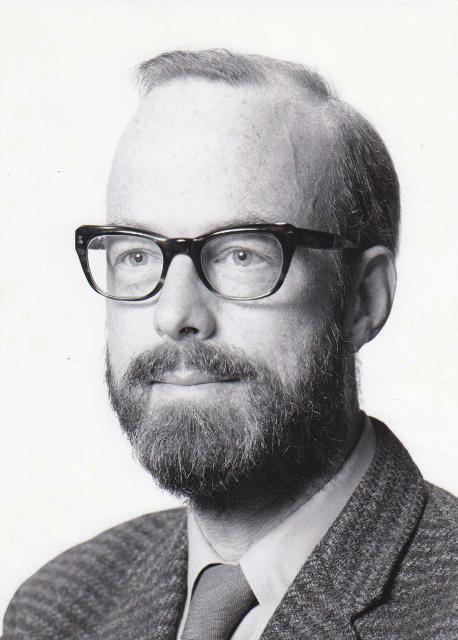
\includegraphics{Tony Hoare.jpg}
    \newline
    \newline
    En 1962, Tony Hoare inventa le tri rapide (Quicksort), qui est généralement considéré comme l'algorithme le plus utilisé dans le monde entier.
\end{center}

\newpage
\tableofcontents

\newpage
\section{Introduction}

\subsection{Définition}

\paragraph{}
Un algorithme de tri est, en informatique ou en mathématiques, un algorithme qui permet d'organiser une collection d'objets selon une relation d'ordre déterminée.
\newline
La collection à trier est souvent donnée sous forme de tableau, afin de permettre l'accès direct aux différents éléments de la collection, ou sous forme de liste, ce qui peut se révéler être plus adapté à certains algorithmes et à l'usage de la programmation fonctionnelle.\\

\paragraph{}
Aujourd'hui on retrouve de nombreux algorithmes de tri que l'on peut diviser en 3 grandes catégories:
\begin{itemize}
    \item Les Tris par comparaison
    \item Les Tris utilisant la structure de données
    \item Les Tris externes
\end{itemize}
\vspace{0.5cm}
Les tris par comparaison peuvent encore se diviser en 4 sous catégories en fonction de leur vitesse d'exécution:

\vspace{0.2cm}
\begin{itemize}
    \item Les algorithmes rapides avec une complexité moyenne de $n*\log(n)$
    \item Les algorithmes moyennement rapides (En moyenne O($n^2$), O(n) dans le meilleur des cas)
    \item Les algorithmes lents avec une complexité de O($n^2$) dans tous les cas
    \item Les algorithmes très lents avec une complexité moyenne moins bonne que O($n^2$)
\end{itemize}

\subsection{Exemples}
\subsubsection{Les Tris par comparaison}
\begin{itemize}
    \item Le tri fusion (dit merge sort)
    \item Le tri rapide (dit quicksort)
    \item Le tri par tas (dit heap sort)
    \item Le tri fusion (dit merge sort)
    \item Le tri par insertion
    \item Le tri à bulle
    \item Le tri par sélection
    \item Le tri stupide
    \item Le tri faire-valoir
\end{itemize}
\newpage
\subsubsection{Les Tris utilisant la structure de données}
\begin{itemize}
    \item Le tri comptage ou tri par dénombrement
    \item Le tri par base
    \item Le tri par paquets
\end{itemize}

\subsubsection{Les Tris externes}
Ces algorithmes sont souvent basés sur une approche assez voisine de celle du tri fusion. Le principe est le suivant :
\vspace{0.2cm}

\begin{itemize}
    \item découpage du volume de données à trier en sous-ensembles de taille inférieure à la mémoire rapide disponible ;
    \item tri de chaque sous-ensemble en mémoire centrale pour former des « monotonies » (sous-ensembles triés) ;
    \item interclassement des monotonies.
\end{itemize}

\section{Critères de classification}
La classification des algorithmes de tri est très importante, car elle permet de choisir l’algorithme le plus adapté au problème traité, tout en tenant compte des contraintes imposées par celui-ci. Les principales caractéristiques qui permettent de différencier les algorithmes de tri, outre leur principe de fonctionnement, sont la complexité temporelle, la complexité spatiale et le caractère stable.
\subsection{Principe de fonctionnement}


\newpage
\subsection{Complexité algorithmique}
Afin d’évaluer la complexité des différents algorithmes de tri présentés,
on comptera le nombre de comparaisons et d’échanges de valeur entre deux
éléments du tableau sans prendre en compte les affectations et comparaisons
sur des variables de comptage de boucles.\\
\vspace{0.1cm}

Les méthodes présentées sont de deux types :
\begin{itemize}
    \item des méthodes qui trient les éléments deux à deux, de manière plus ou moins
          efficace, mais qui nécessitent toujours de comparer chacun des N éléments avec
          chacun des N-1 autres éléments, donc le nombre de comparaisons sera de l’ordre
          de $n^2$ — on note cet ordre de grandeur \displaystyle O($n^2$).
          \vspace{0.1cm}

          Par exemple, pour n=1000, $n^2$=$10^6$, pour n=$10^6$, $n^2$=$10^{12}$.
          \vspace{0.2cm}

          Les algorithmes de ce type sont :
          \begin{itemize}
              \item une méthode de tri élémentaire, le tri par sélection ;
              \item et sa variante, le tri par propagation ou tri bulle ;
              \item une méthode qui s’apparente à celle utilisée pour trier ses cartes dans un jeu,
                    le tri par insertion ;
          \end{itemize}
          \vspace{0.2cm}

    \item des des méthodes qui sont plus rapides, car elles trient des sous-ensembles de ces N éléments puis regroupent les
          éléments triés, elles illustrent le principe « diviser pour régner ». Le nombre de comparaisons est alors de l’ordre de
          $n*\log(n)$.
          \vspace{0.1cm}

          Par exemple, pour n=1000, $n*\log(n)$=10000 environ, pour {n=$10^6$}, $n*\log(n)$=$20*10^6$ environ.
          \vspace{0.2cm}

          Les algorithmes de ce type sont :
          \begin{itemize}

              \item le fameux tri rapide ou Quicksort ;
              \item et enfin, le tri par fusion.
          \end{itemize}
          \vspace{0.1cm}

          Cette liste n’est évidemment pas exhaustive. Il existe des méthodes particulièrement adaptées à certains types de données spécifiques. Le tri par base (dit radix sort) en est un exemple.
          \newline
          \newline
          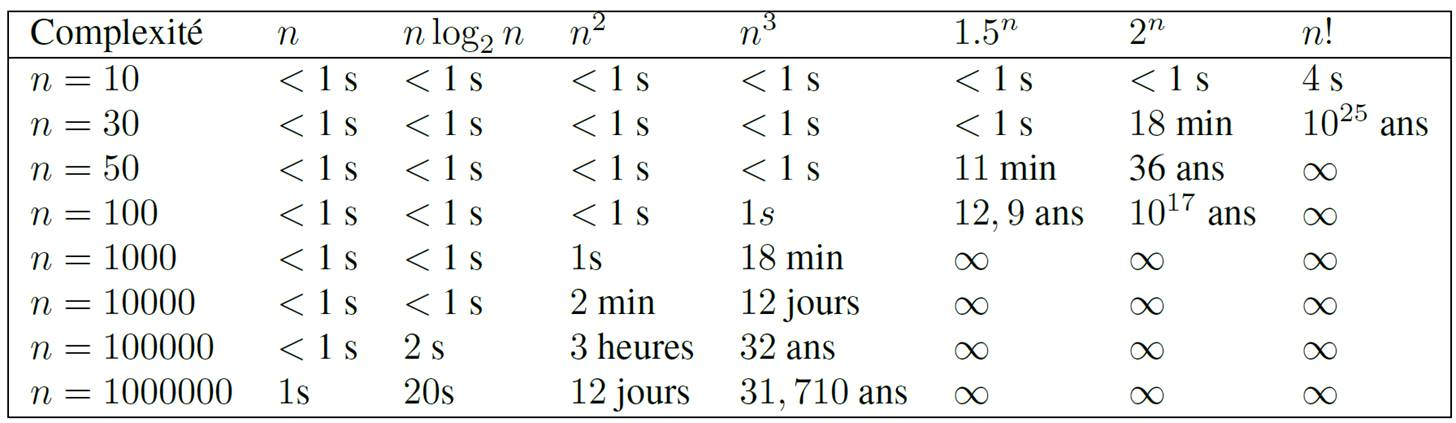
\includegraphics[scale = 0.5]{O(n).jpg}
          \underline {Temps d'éxécution en fonction de la compléxité et du nombre d'éléments}


\end{itemize}

\subsection{Complexité spatiale}

\subsection{Tri en place}

\subsection{Tri stable}

\subsection{Tri interne et externe}

\subsection{Tri parallèle}

\section{Présentation des tris}

\section{Comparaison des algorithmes}
\subsection{Lien avec les données}
L’étude théorique des algorithmes n’est pas suffisante car l’efficacité de ces-derniers dépend
aussi de l’ordre des données sur lesquelles on les utilise. Les algorithmes que nous allons considérés
par la suite sont les tris : \textit{par tas}, \textit{compte}, \textit{fusion} et \textit{rapide}. Pour les étudier et les
comparer, on se propose de créer plusieurs ensembles de données.
On ordonnera les données toujours par ordre croissant. De plus, on donnera aux données un
ordre prédéfini (avant le tri). Les jeux de données seront ordonnés : par ordre croissant de 0 à n,
par ordre décroissant de n à 0 (inversé), aléatoirement sans redondance de donnée, aléatoirement
avec redondance, aléatoirement mais de façon uniforme sans redondance et aléatoirement de façon
uniforme mais avec redondance. D’autre part, on fera varié la taille de ces jeux de données (on
aura par exemple n = 10, n = 500, n = 25000).

\section{Conclusion}

\end{document}